\documentclass[twoside]{book}

% Packages required by doxygen
\usepackage{calc}
\usepackage{doxygen}
\usepackage{graphicx}
\usepackage[utf8]{inputenc}
\usepackage{makeidx}
\usepackage{multicol}
\usepackage{multirow}
\usepackage{textcomp}
\usepackage[table]{xcolor}

% Font selection
\usepackage[T1]{fontenc}
\usepackage{mathptmx}
\usepackage[scaled=.90]{helvet}
\usepackage{courier}
\usepackage{amssymb}
\usepackage{sectsty}
\renewcommand{\familydefault}{\sfdefault}
\allsectionsfont{%
  \fontseries{bc}\selectfont%
  \color{darkgray}%
}
\renewcommand{\DoxyLabelFont}{%
  \fontseries{bc}\selectfont%
  \color{darkgray}%
}

% Page & text layout
\usepackage{geometry}
\geometry{%
  a4paper,%
  top=2.5cm,%
  bottom=2.5cm,%
  left=2.5cm,%
  right=2.5cm%
}
\tolerance=750
\hfuzz=15pt
\hbadness=750
\setlength{\emergencystretch}{15pt}
\setlength{\parindent}{0cm}
\setlength{\parskip}{0.2cm}
\makeatletter
\renewcommand{\paragraph}{%
  \@startsection{paragraph}{4}{0ex}{-1.0ex}{1.0ex}{%
    \normalfont\normalsize\bfseries\SS@parafont%
  }%
}
\renewcommand{\subparagraph}{%
  \@startsection{subparagraph}{5}{0ex}{-1.0ex}{1.0ex}{%
    \normalfont\normalsize\bfseries\SS@subparafont%
  }%
}
\makeatother

% Headers & footers
\usepackage{fancyhdr}
\pagestyle{fancyplain}
\fancyhead[LE]{\fancyplain{}{\bfseries\thepage}}
\fancyhead[CE]{\fancyplain{}{}}
\fancyhead[RE]{\fancyplain{}{\bfseries\leftmark}}
\fancyhead[LO]{\fancyplain{}{\bfseries\rightmark}}
\fancyhead[CO]{\fancyplain{}{}}
\fancyhead[RO]{\fancyplain{}{\bfseries\thepage}}
\fancyfoot[LE]{\fancyplain{}{}}
\fancyfoot[CE]{\fancyplain{}{}}
\fancyfoot[RE]{\fancyplain{}{\bfseries\scriptsize Generated on Tue Jul 28 2015 13\-:17\-:56 for My Project by Doxygen }}
\fancyfoot[LO]{\fancyplain{}{\bfseries\scriptsize Generated on Tue Jul 28 2015 13\-:17\-:56 for My Project by Doxygen }}
\fancyfoot[CO]{\fancyplain{}{}}
\fancyfoot[RO]{\fancyplain{}{}}
\renewcommand{\footrulewidth}{0.4pt}
\renewcommand{\chaptermark}[1]{%
  \markboth{#1}{}%
}
\renewcommand{\sectionmark}[1]{%
  \markright{\thesection\ #1}%
}

% Indices & bibliography
\usepackage{natbib}
\usepackage[titles]{tocloft}
\setcounter{tocdepth}{3}
\setcounter{secnumdepth}{5}
\makeindex

% Hyperlinks (required, but should be loaded last)
\usepackage{ifpdf}
\ifpdf
  \usepackage[pdftex,pagebackref=true]{hyperref}
\else
  \usepackage[ps2pdf,pagebackref=true]{hyperref}
\fi
\hypersetup{%
  colorlinks=true,%
  linkcolor=blue,%
  citecolor=blue,%
  unicode%
}

% Custom commands
\newcommand{\clearemptydoublepage}{%
  \newpage{\pagestyle{empty}\cleardoublepage}%
}


%===== C O N T E N T S =====

\begin{document}

% Titlepage & ToC
\hypersetup{pageanchor=false}
\pagenumbering{roman}
\begin{titlepage}
\vspace*{7cm}
\begin{center}%
{\Large My Project }\\
\vspace*{1cm}
{\large Generated by Doxygen 1.8.6}\\
\vspace*{0.5cm}
{\small Tue Jul 28 2015 13:17:56}\\
\end{center}
\end{titlepage}
\clearemptydoublepage
\tableofcontents
\clearemptydoublepage
\pagenumbering{arabic}
\hypersetup{pageanchor=true}

%--- Begin generated contents ---
\chapter{Namespace Index}
\section{Namespace List}
Here is a list of all namespaces with brief descriptions\-:\begin{DoxyCompactList}
\item\contentsline{section}{\hyperlink{namespaceAutoTest}{Auto\-Test} }{\pageref{namespaceAutoTest}}{}
\end{DoxyCompactList}

\chapter{Hierarchical Index}
\section{Class Hierarchy}
This inheritance list is sorted roughly, but not completely, alphabetically\-:\begin{DoxyCompactList}
\item \contentsline{section}{Coords}{\pageref{classCoords}}{}
\item Q\-Object\begin{DoxyCompactList}
\item \contentsline{section}{Test\-Coord}{\pageref{classTestCoord}}{}
\item \contentsline{section}{Test\-Radar}{\pageref{classTestRadar}}{}
\end{DoxyCompactList}
\item \contentsline{section}{Radar}{\pageref{classRadar}}{}
\item \contentsline{section}{Test$<$ T $>$}{\pageref{classTest}}{}
\end{DoxyCompactList}

\chapter{Class Index}
\section{Class List}
Here are the classes, structs, unions and interfaces with brief descriptions\-:\begin{DoxyCompactList}
\item\contentsline{section}{\hyperlink{classCoords}{Coords} \\*Trieda \hyperlink{classCoords}{Coords} }{\pageref{classCoords}}{}
\item\contentsline{section}{\hyperlink{classRadar}{Radar} \\*Trieda \hyperlink{classRadar}{Radar} }{\pageref{classRadar}}{}
\item\contentsline{section}{\hyperlink{classTest}{Test$<$ T $>$} }{\pageref{classTest}}{}
\item\contentsline{section}{\hyperlink{classTestCoord}{Test\-Coord} }{\pageref{classTestCoord}}{}
\item\contentsline{section}{\hyperlink{classTestRadar}{Test\-Radar} }{\pageref{classTestRadar}}{}
\end{DoxyCompactList}

\chapter{File Index}
\section{File List}
Here is a list of all files with brief descriptions\-:\begin{DoxyCompactList}
\item\contentsline{section}{\hyperlink{AutoTest_8h}{Auto\-Test.\-h} }{\pageref{AutoTest_8h}}{}
\item\contentsline{section}{\hyperlink{coords_8cpp}{coords.\-cpp} \\*Tento subor obsahuje konstruktor a metody triedy \hyperlink{classCoords}{Coords} predstavujuce suradnice radaroveho systemu }{\pageref{coords_8cpp}}{}
\item\contentsline{section}{\hyperlink{coords_8h}{coords.\-h} }{\pageref{coords_8h}}{}
\item\contentsline{section}{\hyperlink{main_8cpp}{main.\-cpp} }{\pageref{main_8cpp}}{}
\item\contentsline{section}{\hyperlink{radar_8cpp}{radar.\-cpp} }{\pageref{radar_8cpp}}{}
\item\contentsline{section}{\hyperlink{radar_8h}{radar.\-h} }{\pageref{radar_8h}}{}
\item\contentsline{section}{\hyperlink{test__coord_8cpp}{test\-\_\-coord.\-cpp} }{\pageref{test__coord_8cpp}}{}
\item\contentsline{section}{\hyperlink{test__coord_8h}{test\-\_\-coord.\-h} }{\pageref{test__coord_8h}}{}
\item\contentsline{section}{\hyperlink{test__radar_8cpp}{test\-\_\-radar.\-cpp} }{\pageref{test__radar_8cpp}}{}
\item\contentsline{section}{\hyperlink{test__radar_8h}{test\-\_\-radar.\-h} }{\pageref{test__radar_8h}}{}
\end{DoxyCompactList}

\chapter{Namespace Documentation}
\hypertarget{namespaceAutoTest}{\section{Auto\-Test Namespace Reference}
\label{namespaceAutoTest}\index{Auto\-Test@{Auto\-Test}}
}
\subsection*{Typedefs}
\begin{DoxyCompactItemize}
\item 
typedef Q\-List$<$ Q\-Object $\ast$ $>$ \hyperlink{namespaceAutoTest_af30e241e62927ef8b429177cea542f2f}{Test\-List}
\end{DoxyCompactItemize}
\subsection*{Functions}
\begin{DoxyCompactItemize}
\item 
\hyperlink{namespaceAutoTest_af30e241e62927ef8b429177cea542f2f}{Test\-List} \& \hyperlink{namespaceAutoTest_ad402cc96e71645ac9d583473f7ddbcd7}{test\-List} ()
\item 
bool \hyperlink{namespaceAutoTest_aebe87b1ec91a09f1b2739cbd4b301345}{find\-Object} (Q\-Object $\ast$object)
\item 
void \hyperlink{namespaceAutoTest_a3d2e7034d932dff0c2ba4170c442f594}{add\-Test} (Q\-Object $\ast$object)
\item 
int \hyperlink{namespaceAutoTest_a3261ec6bff9391a6f6779f63f6663b4b}{run} (int argc, char $\ast$argv\mbox{[}$\,$\mbox{]})
\end{DoxyCompactItemize}


\subsection{Typedef Documentation}
\hypertarget{namespaceAutoTest_af30e241e62927ef8b429177cea542f2f}{\index{Auto\-Test@{Auto\-Test}!Test\-List@{Test\-List}}
\index{Test\-List@{Test\-List}!AutoTest@{Auto\-Test}}
\subsubsection[{Test\-List}]{\setlength{\rightskip}{0pt plus 5cm}typedef Q\-List$<$Q\-Object$\ast$$>$ {\bf Auto\-Test\-::\-Test\-List}}}\label{namespaceAutoTest_af30e241e62927ef8b429177cea542f2f}


\subsection{Function Documentation}
\hypertarget{namespaceAutoTest_a3d2e7034d932dff0c2ba4170c442f594}{\index{Auto\-Test@{Auto\-Test}!add\-Test@{add\-Test}}
\index{add\-Test@{add\-Test}!AutoTest@{Auto\-Test}}
\subsubsection[{add\-Test}]{\setlength{\rightskip}{0pt plus 5cm}void Auto\-Test\-::add\-Test (
\begin{DoxyParamCaption}
\item[{Q\-Object $\ast$}]{object}
\end{DoxyParamCaption}
)\hspace{0.3cm}{\ttfamily [inline]}}}\label{namespaceAutoTest_a3d2e7034d932dff0c2ba4170c442f594}


Here is the call graph for this function\-:
\nopagebreak
\begin{figure}[H]
\begin{center}
\leavevmode
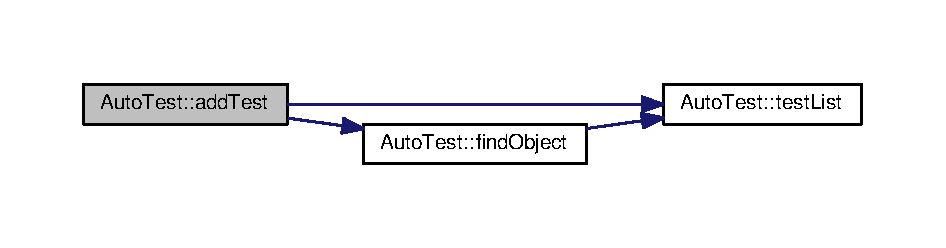
\includegraphics[width=350pt]{namespaceAutoTest_a3d2e7034d932dff0c2ba4170c442f594_cgraph}
\end{center}
\end{figure}


\hypertarget{namespaceAutoTest_aebe87b1ec91a09f1b2739cbd4b301345}{\index{Auto\-Test@{Auto\-Test}!find\-Object@{find\-Object}}
\index{find\-Object@{find\-Object}!AutoTest@{Auto\-Test}}
\subsubsection[{find\-Object}]{\setlength{\rightskip}{0pt plus 5cm}bool Auto\-Test\-::find\-Object (
\begin{DoxyParamCaption}
\item[{Q\-Object $\ast$}]{object}
\end{DoxyParamCaption}
)\hspace{0.3cm}{\ttfamily [inline]}}}\label{namespaceAutoTest_aebe87b1ec91a09f1b2739cbd4b301345}


Here is the call graph for this function\-:
\nopagebreak
\begin{figure}[H]
\begin{center}
\leavevmode
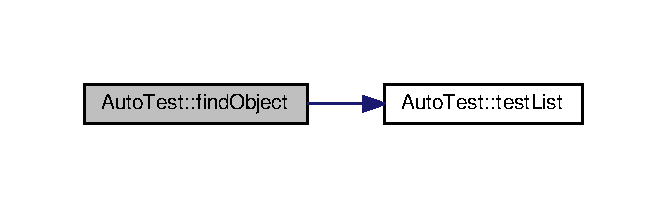
\includegraphics[width=320pt]{namespaceAutoTest_aebe87b1ec91a09f1b2739cbd4b301345_cgraph}
\end{center}
\end{figure}


\hypertarget{namespaceAutoTest_a3261ec6bff9391a6f6779f63f6663b4b}{\index{Auto\-Test@{Auto\-Test}!run@{run}}
\index{run@{run}!AutoTest@{Auto\-Test}}
\subsubsection[{run}]{\setlength{\rightskip}{0pt plus 5cm}int Auto\-Test\-::run (
\begin{DoxyParamCaption}
\item[{int}]{argc, }
\item[{char $\ast$}]{argv\mbox{[}$\,$\mbox{]}}
\end{DoxyParamCaption}
)\hspace{0.3cm}{\ttfamily [inline]}}}\label{namespaceAutoTest_a3261ec6bff9391a6f6779f63f6663b4b}


Here is the call graph for this function\-:
\nopagebreak
\begin{figure}[H]
\begin{center}
\leavevmode
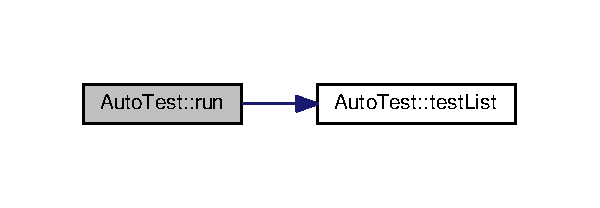
\includegraphics[width=288pt]{namespaceAutoTest_a3261ec6bff9391a6f6779f63f6663b4b_cgraph}
\end{center}
\end{figure}


\hypertarget{namespaceAutoTest_ad402cc96e71645ac9d583473f7ddbcd7}{\index{Auto\-Test@{Auto\-Test}!test\-List@{test\-List}}
\index{test\-List@{test\-List}!AutoTest@{Auto\-Test}}
\subsubsection[{test\-List}]{\setlength{\rightskip}{0pt plus 5cm}{\bf Test\-List}\& Auto\-Test\-::test\-List (
\begin{DoxyParamCaption}
{}
\end{DoxyParamCaption}
)\hspace{0.3cm}{\ttfamily [inline]}}}\label{namespaceAutoTest_ad402cc96e71645ac9d583473f7ddbcd7}

\chapter{Class Documentation}
\hypertarget{classCoords}{\section{Coords Class Reference}
\label{classCoords}\index{Coords@{Coords}}
}


Trieda \hyperlink{classCoords}{Coords}.  




{\ttfamily \#include $<$coords.\-h$>$}

\subsection*{Public Member Functions}
\begin{DoxyCompactItemize}
\item 
\hyperlink{classCoords_a5922d1783cefa759950faa50ac347191}{Coords} ()
\item 
\hyperlink{classCoords_a370c5fad753558f68cfe993ccfa6aefc}{Coords} (double, double, double, double, double, double)
\item 
void \hyperlink{classCoords_a0bf0acf0cddd3ca2d010adf98400bb12}{set\-Latitude\-D} (double)
\item 
void \hyperlink{classCoords_ad0384a14a8c3665c367723574ed6c145}{set\-Latitude\-M} (double)
\item 
void \hyperlink{classCoords_ab87a774c4b6eff3abf498a39e767c416}{set\-Latitude\-S} (double)
\item 
void \hyperlink{classCoords_a8d32d6e7a46e5754120f9024c27df7a5}{set\-Longitude\-D} (double)
\item 
void \hyperlink{classCoords_a7d54f335e89544d1f1cdab70eebc6fed}{set\-Longitude\-M} (double)
\item 
void \hyperlink{classCoords_a5c2ac2d68dee771445b953e158bc5505}{set\-Longitude\-S} (double)
\item 
void \hyperlink{classCoords_a6733bf6813065b00d254830f2f02315b}{set\-Dec\-Latitude} (double dec\-Latitude)
\item 
void \hyperlink{classCoords_acfe86d1cd0160163dee9119e03a78438}{set\-Dec\-Longitude} (double dec\-Longitude)
\item 
double \hyperlink{classCoords_af48729f8925b858e242c630261ed0859}{get\-Latitude\-D} (void)
\item 
double \hyperlink{classCoords_a4c836418545be6776c65806286e62084}{get\-Latitude\-M} (void)
\item 
double \hyperlink{classCoords_aa73a7700f91f4075638071787b08dd2e}{get\-Latitude\-S} (void)
\item 
double \hyperlink{classCoords_a34dffdf0fa5b6f8b7c68abcaa3c947c9}{get\-Longitude\-D} (void)
\item 
double \hyperlink{classCoords_a219e69414cb772e743f2ce64060eeac1}{get\-Longitude\-M} (void)
\item 
double \hyperlink{classCoords_a75827c87b5718c36f6c8df091e9d025f}{get\-Longitude\-S} (void)
\item 
double \hyperlink{classCoords_a9cbddbe1650244f71f2accb3a8c6db4c}{get\-Dec\-Latitude} ()
\item 
double \hyperlink{classCoords_a1d965b74b2bae7532f128d790de19f4b}{get\-Dec\-Longitude} ()
\item 
void \hyperlink{classCoords_ab7b884f80b3327d5fec4ca379abb92d8}{Deg\-To\-Dec} (void)
\end{DoxyCompactItemize}


\subsection{Detailed Description}
Trieda \hyperlink{classCoords}{Coords}. 

Trieda \hyperlink{classCoords}{Coords} predstavuje suradnice radaroveho systemu a ich prevod do roznych typov. 

\subsection{Constructor \& Destructor Documentation}
\hypertarget{classCoords_a5922d1783cefa759950faa50ac347191}{\index{Coords@{Coords}!Coords@{Coords}}
\index{Coords@{Coords}!Coords@{Coords}}
\subsubsection[{Coords}]{\setlength{\rightskip}{0pt plus 5cm}Coords\-::\-Coords (
\begin{DoxyParamCaption}
{}
\end{DoxyParamCaption}
)}}\label{classCoords_a5922d1783cefa759950faa50ac347191}
Impicitny konstruktor \hypertarget{classCoords_a370c5fad753558f68cfe993ccfa6aefc}{\index{Coords@{Coords}!Coords@{Coords}}
\index{Coords@{Coords}!Coords@{Coords}}
\subsubsection[{Coords}]{\setlength{\rightskip}{0pt plus 5cm}Coords\-::\-Coords (
\begin{DoxyParamCaption}
\item[{double}]{latitude\-D, }
\item[{double}]{latitude\-M, }
\item[{double}]{latitude\-S, }
\item[{double}]{longitude\-D, }
\item[{double}]{longitude\-M, }
\item[{double}]{longitude\-S}
\end{DoxyParamCaption}
)}}\label{classCoords_a370c5fad753558f68cfe993ccfa6aefc}
Konstruktor triedy \hyperlink{classCoords}{Coords} obsahujuci vstupne suradnice.

Konstruktor ma ako vstupne argumenty sestticu cisel predstavujucich stupne minuty a sekundy zemepisnej sirky a dlzky.


\begin{DoxyParams}{Parameters}
{\em array\-Size} & size of dynamically allocated array \\
\hline
\end{DoxyParams}
\begin{DoxyReturn}{Returns}
nothing 
\end{DoxyReturn}
$<$ Informacia o stupni zemepisnej sirky

$<$ Informacia o minute zemepisnej sirky

$<$ Informacia o sekunde zemepisnej sirky

$<$ Informacia o stupni zemepisnej dlzky

$<$ Informacia o stupni zemepisnej dlzky

$<$ Informacia o stupni zemepisnej dlzky

$<$ Prevod zemepisnej sirky do dekadickych stupnov

$<$ Prevod zemepisnej dlzky do dekadickych stupnov 

Here is the call graph for this function\-:
\nopagebreak
\begin{figure}[H]
\begin{center}
\leavevmode
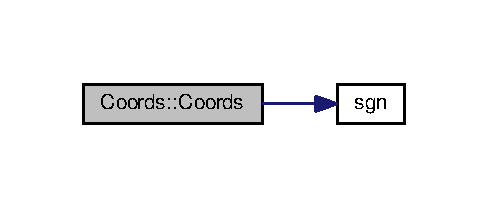
\includegraphics[width=234pt]{classCoords_a370c5fad753558f68cfe993ccfa6aefc_cgraph}
\end{center}
\end{figure}




\subsection{Member Function Documentation}
\hypertarget{classCoords_ab7b884f80b3327d5fec4ca379abb92d8}{\index{Coords@{Coords}!Deg\-To\-Dec@{Deg\-To\-Dec}}
\index{Deg\-To\-Dec@{Deg\-To\-Dec}!Coords@{Coords}}
\subsubsection[{Deg\-To\-Dec}]{\setlength{\rightskip}{0pt plus 5cm}void Coords\-::\-Deg\-To\-Dec (
\begin{DoxyParamCaption}
\item[{void}]{}
\end{DoxyParamCaption}
)}}\label{classCoords_ab7b884f80b3327d5fec4ca379abb92d8}
\hypertarget{classCoords_a9cbddbe1650244f71f2accb3a8c6db4c}{\index{Coords@{Coords}!get\-Dec\-Latitude@{get\-Dec\-Latitude}}
\index{get\-Dec\-Latitude@{get\-Dec\-Latitude}!Coords@{Coords}}
\subsubsection[{get\-Dec\-Latitude}]{\setlength{\rightskip}{0pt plus 5cm}double Coords\-::get\-Dec\-Latitude (
\begin{DoxyParamCaption}
{}
\end{DoxyParamCaption}
)}}\label{classCoords_a9cbddbe1650244f71f2accb3a8c6db4c}
\hypertarget{classCoords_a1d965b74b2bae7532f128d790de19f4b}{\index{Coords@{Coords}!get\-Dec\-Longitude@{get\-Dec\-Longitude}}
\index{get\-Dec\-Longitude@{get\-Dec\-Longitude}!Coords@{Coords}}
\subsubsection[{get\-Dec\-Longitude}]{\setlength{\rightskip}{0pt plus 5cm}double Coords\-::get\-Dec\-Longitude (
\begin{DoxyParamCaption}
{}
\end{DoxyParamCaption}
)}}\label{classCoords_a1d965b74b2bae7532f128d790de19f4b}
\hypertarget{classCoords_af48729f8925b858e242c630261ed0859}{\index{Coords@{Coords}!get\-Latitude\-D@{get\-Latitude\-D}}
\index{get\-Latitude\-D@{get\-Latitude\-D}!Coords@{Coords}}
\subsubsection[{get\-Latitude\-D}]{\setlength{\rightskip}{0pt plus 5cm}double Coords\-::get\-Latitude\-D (
\begin{DoxyParamCaption}
\item[{void}]{}
\end{DoxyParamCaption}
)}}\label{classCoords_af48729f8925b858e242c630261ed0859}
\hypertarget{classCoords_a4c836418545be6776c65806286e62084}{\index{Coords@{Coords}!get\-Latitude\-M@{get\-Latitude\-M}}
\index{get\-Latitude\-M@{get\-Latitude\-M}!Coords@{Coords}}
\subsubsection[{get\-Latitude\-M}]{\setlength{\rightskip}{0pt plus 5cm}double Coords\-::get\-Latitude\-M (
\begin{DoxyParamCaption}
\item[{void}]{}
\end{DoxyParamCaption}
)}}\label{classCoords_a4c836418545be6776c65806286e62084}
\hypertarget{classCoords_aa73a7700f91f4075638071787b08dd2e}{\index{Coords@{Coords}!get\-Latitude\-S@{get\-Latitude\-S}}
\index{get\-Latitude\-S@{get\-Latitude\-S}!Coords@{Coords}}
\subsubsection[{get\-Latitude\-S}]{\setlength{\rightskip}{0pt plus 5cm}double Coords\-::get\-Latitude\-S (
\begin{DoxyParamCaption}
\item[{void}]{}
\end{DoxyParamCaption}
)}}\label{classCoords_aa73a7700f91f4075638071787b08dd2e}
\hypertarget{classCoords_a34dffdf0fa5b6f8b7c68abcaa3c947c9}{\index{Coords@{Coords}!get\-Longitude\-D@{get\-Longitude\-D}}
\index{get\-Longitude\-D@{get\-Longitude\-D}!Coords@{Coords}}
\subsubsection[{get\-Longitude\-D}]{\setlength{\rightskip}{0pt plus 5cm}double Coords\-::get\-Longitude\-D (
\begin{DoxyParamCaption}
\item[{void}]{}
\end{DoxyParamCaption}
)}}\label{classCoords_a34dffdf0fa5b6f8b7c68abcaa3c947c9}
\hypertarget{classCoords_a219e69414cb772e743f2ce64060eeac1}{\index{Coords@{Coords}!get\-Longitude\-M@{get\-Longitude\-M}}
\index{get\-Longitude\-M@{get\-Longitude\-M}!Coords@{Coords}}
\subsubsection[{get\-Longitude\-M}]{\setlength{\rightskip}{0pt plus 5cm}double Coords\-::get\-Longitude\-M (
\begin{DoxyParamCaption}
\item[{void}]{}
\end{DoxyParamCaption}
)}}\label{classCoords_a219e69414cb772e743f2ce64060eeac1}
\hypertarget{classCoords_a75827c87b5718c36f6c8df091e9d025f}{\index{Coords@{Coords}!get\-Longitude\-S@{get\-Longitude\-S}}
\index{get\-Longitude\-S@{get\-Longitude\-S}!Coords@{Coords}}
\subsubsection[{get\-Longitude\-S}]{\setlength{\rightskip}{0pt plus 5cm}double Coords\-::get\-Longitude\-S (
\begin{DoxyParamCaption}
\item[{void}]{}
\end{DoxyParamCaption}
)}}\label{classCoords_a75827c87b5718c36f6c8df091e9d025f}
\hypertarget{classCoords_a6733bf6813065b00d254830f2f02315b}{\index{Coords@{Coords}!set\-Dec\-Latitude@{set\-Dec\-Latitude}}
\index{set\-Dec\-Latitude@{set\-Dec\-Latitude}!Coords@{Coords}}
\subsubsection[{set\-Dec\-Latitude}]{\setlength{\rightskip}{0pt plus 5cm}void Coords\-::set\-Dec\-Latitude (
\begin{DoxyParamCaption}
\item[{double}]{dec\-Latitude}
\end{DoxyParamCaption}
)}}\label{classCoords_a6733bf6813065b00d254830f2f02315b}
\hypertarget{classCoords_acfe86d1cd0160163dee9119e03a78438}{\index{Coords@{Coords}!set\-Dec\-Longitude@{set\-Dec\-Longitude}}
\index{set\-Dec\-Longitude@{set\-Dec\-Longitude}!Coords@{Coords}}
\subsubsection[{set\-Dec\-Longitude}]{\setlength{\rightskip}{0pt plus 5cm}void Coords\-::set\-Dec\-Longitude (
\begin{DoxyParamCaption}
\item[{double}]{dec\-Longitude}
\end{DoxyParamCaption}
)}}\label{classCoords_acfe86d1cd0160163dee9119e03a78438}
\hypertarget{classCoords_a0bf0acf0cddd3ca2d010adf98400bb12}{\index{Coords@{Coords}!set\-Latitude\-D@{set\-Latitude\-D}}
\index{set\-Latitude\-D@{set\-Latitude\-D}!Coords@{Coords}}
\subsubsection[{set\-Latitude\-D}]{\setlength{\rightskip}{0pt plus 5cm}void Coords\-::set\-Latitude\-D (
\begin{DoxyParamCaption}
\item[{double}]{latitude\-D}
\end{DoxyParamCaption}
)}}\label{classCoords_a0bf0acf0cddd3ca2d010adf98400bb12}
\hypertarget{classCoords_ad0384a14a8c3665c367723574ed6c145}{\index{Coords@{Coords}!set\-Latitude\-M@{set\-Latitude\-M}}
\index{set\-Latitude\-M@{set\-Latitude\-M}!Coords@{Coords}}
\subsubsection[{set\-Latitude\-M}]{\setlength{\rightskip}{0pt plus 5cm}void Coords\-::set\-Latitude\-M (
\begin{DoxyParamCaption}
\item[{double}]{latitude\-M}
\end{DoxyParamCaption}
)}}\label{classCoords_ad0384a14a8c3665c367723574ed6c145}
\hypertarget{classCoords_ab87a774c4b6eff3abf498a39e767c416}{\index{Coords@{Coords}!set\-Latitude\-S@{set\-Latitude\-S}}
\index{set\-Latitude\-S@{set\-Latitude\-S}!Coords@{Coords}}
\subsubsection[{set\-Latitude\-S}]{\setlength{\rightskip}{0pt plus 5cm}void Coords\-::set\-Latitude\-S (
\begin{DoxyParamCaption}
\item[{double}]{latitude\-S}
\end{DoxyParamCaption}
)}}\label{classCoords_ab87a774c4b6eff3abf498a39e767c416}
\hypertarget{classCoords_a8d32d6e7a46e5754120f9024c27df7a5}{\index{Coords@{Coords}!set\-Longitude\-D@{set\-Longitude\-D}}
\index{set\-Longitude\-D@{set\-Longitude\-D}!Coords@{Coords}}
\subsubsection[{set\-Longitude\-D}]{\setlength{\rightskip}{0pt plus 5cm}void Coords\-::set\-Longitude\-D (
\begin{DoxyParamCaption}
\item[{double}]{longitude\-D}
\end{DoxyParamCaption}
)}}\label{classCoords_a8d32d6e7a46e5754120f9024c27df7a5}
\hypertarget{classCoords_a7d54f335e89544d1f1cdab70eebc6fed}{\index{Coords@{Coords}!set\-Longitude\-M@{set\-Longitude\-M}}
\index{set\-Longitude\-M@{set\-Longitude\-M}!Coords@{Coords}}
\subsubsection[{set\-Longitude\-M}]{\setlength{\rightskip}{0pt plus 5cm}void Coords\-::set\-Longitude\-M (
\begin{DoxyParamCaption}
\item[{double}]{longitude\-M}
\end{DoxyParamCaption}
)}}\label{classCoords_a7d54f335e89544d1f1cdab70eebc6fed}
\hypertarget{classCoords_a5c2ac2d68dee771445b953e158bc5505}{\index{Coords@{Coords}!set\-Longitude\-S@{set\-Longitude\-S}}
\index{set\-Longitude\-S@{set\-Longitude\-S}!Coords@{Coords}}
\subsubsection[{set\-Longitude\-S}]{\setlength{\rightskip}{0pt plus 5cm}void Coords\-::set\-Longitude\-S (
\begin{DoxyParamCaption}
\item[{double}]{longitude\-S}
\end{DoxyParamCaption}
)}}\label{classCoords_a5c2ac2d68dee771445b953e158bc5505}


The documentation for this class was generated from the following files\-:\begin{DoxyCompactItemize}
\item 
\hyperlink{coords_8h}{coords.\-h}\item 
\hyperlink{coords_8cpp}{coords.\-cpp}\end{DoxyCompactItemize}

\hypertarget{classRadar}{\section{Radar Class Reference}
\label{classRadar}\index{Radar@{Radar}}
}


Trieda \hyperlink{classRadar}{Radar}.  




{\ttfamily \#include $<$radar.\-h$>$}



Collaboration diagram for Radar\-:
\nopagebreak
\begin{figure}[H]
\begin{center}
\leavevmode
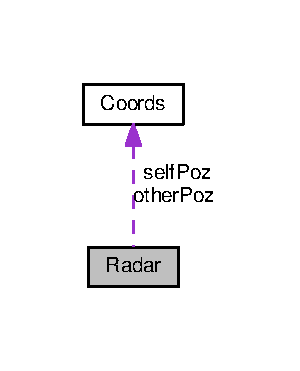
\includegraphics[width=144pt]{classRadar__coll__graph}
\end{center}
\end{figure}
\subsection*{Public Member Functions}
\begin{DoxyCompactItemize}
\item 
\hyperlink{classRadar_a7b410a3b89ddce8d0cd887cec9a68e4c}{Radar} (\hyperlink{classCoords}{Coords}, \hyperlink{classCoords}{Coords})
\item 
double \hyperlink{classRadar_acd5a884b01ca6a2f63fd2e09a2521709}{get\-Distance} (void)
\end{DoxyCompactItemize}
\subsection*{Public Attributes}
\begin{DoxyCompactItemize}
\item 
const double \hyperlink{classRadar_ab545a02c2a5d688cb520115fc0e4dcf4}{sac} =48.\-0
\item 
double \hyperlink{classRadar_a462d860ac5b4af6246074aae7082c94c}{direct\-Distance}
\item 
\hyperlink{classCoords}{Coords} \hyperlink{classRadar_a2475d8141970088a5a6aa92eb0f6535d}{self\-Poz}
\item 
\hyperlink{classCoords}{Coords} \hyperlink{classRadar_aed5172c436c4a1803d6d9f978f3eee02}{other\-Poz}
\end{DoxyCompactItemize}


\subsection{Detailed Description}
Trieda \hyperlink{classRadar}{Radar}. 

Trieda predstavuje model radaru. 

\subsection{Constructor \& Destructor Documentation}
\hypertarget{classRadar_a7b410a3b89ddce8d0cd887cec9a68e4c}{\index{Radar@{Radar}!Radar@{Radar}}
\index{Radar@{Radar}!Radar@{Radar}}
\subsubsection[{Radar}]{\setlength{\rightskip}{0pt plus 5cm}Radar\-::\-Radar (
\begin{DoxyParamCaption}
\item[{{\bf Coords}}]{self\-Poz, }
\item[{{\bf Coords}}]{other\-Poz}
\end{DoxyParamCaption}
)}}\label{classRadar_a7b410a3b89ddce8d0cd887cec9a68e4c}
Konstruktor triedy \hyperlink{classRadar}{Radar} obsahujuci vlastnu a vzdialenu suradnicu.

Konstruktor ma ako vstupne argumenty dva parametre typu \hyperlink{classCoords}{Coords}.


\begin{DoxyParams}{Parameters}
{\em array\-Size} & size of dynamically allocated array \\
\hline
\end{DoxyParams}
\begin{DoxyReturn}{Returns}
nothing 
\end{DoxyReturn}


\subsection{Member Function Documentation}
\hypertarget{classRadar_acd5a884b01ca6a2f63fd2e09a2521709}{\index{Radar@{Radar}!get\-Distance@{get\-Distance}}
\index{get\-Distance@{get\-Distance}!Radar@{Radar}}
\subsubsection[{get\-Distance}]{\setlength{\rightskip}{0pt plus 5cm}double Radar\-::get\-Distance (
\begin{DoxyParamCaption}
\item[{void}]{}
\end{DoxyParamCaption}
)}}\label{classRadar_acd5a884b01ca6a2f63fd2e09a2521709}
Funkcia get\-Distance triedy \hyperlink{classRadar}{Radar} pocitajuca vzdialenost.

Funkcia pocita vzdialenost pomocou kniznice Geographic\-Lib vytvorenu pre geograficke vypocty. 

Here is the call graph for this function\-:
\nopagebreak
\begin{figure}[H]
\begin{center}
\leavevmode
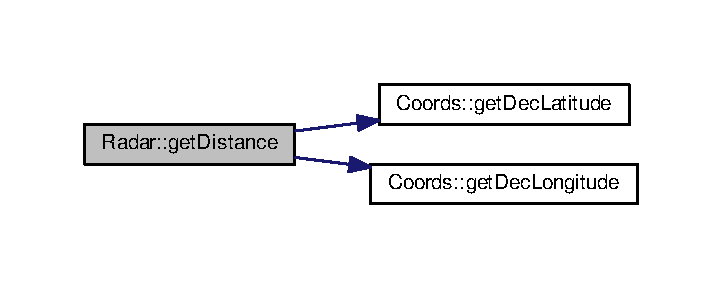
\includegraphics[width=346pt]{classRadar_acd5a884b01ca6a2f63fd2e09a2521709_cgraph}
\end{center}
\end{figure}




\subsection{Member Data Documentation}
\hypertarget{classRadar_a462d860ac5b4af6246074aae7082c94c}{\index{Radar@{Radar}!direct\-Distance@{direct\-Distance}}
\index{direct\-Distance@{direct\-Distance}!Radar@{Radar}}
\subsubsection[{direct\-Distance}]{\setlength{\rightskip}{0pt plus 5cm}double Radar\-::direct\-Distance}}\label{classRadar_a462d860ac5b4af6246074aae7082c94c}
Vzdialenost od inej wgs suradnice \hypertarget{classRadar_aed5172c436c4a1803d6d9f978f3eee02}{\index{Radar@{Radar}!other\-Poz@{other\-Poz}}
\index{other\-Poz@{other\-Poz}!Radar@{Radar}}
\subsubsection[{other\-Poz}]{\setlength{\rightskip}{0pt plus 5cm}{\bf Coords} Radar\-::other\-Poz}}\label{classRadar_aed5172c436c4a1803d6d9f978f3eee02}
Pozicia od ktorej sa pocita vzdialenost \hypertarget{classRadar_ab545a02c2a5d688cb520115fc0e4dcf4}{\index{Radar@{Radar}!sac@{sac}}
\index{sac@{sac}!Radar@{Radar}}
\subsubsection[{sac}]{\setlength{\rightskip}{0pt plus 5cm}const double Radar\-::sac =48.\-0}}\label{classRadar_ab545a02c2a5d688cb520115fc0e4dcf4}
S\-A\-C identifikator \hypertarget{classRadar_a2475d8141970088a5a6aa92eb0f6535d}{\index{Radar@{Radar}!self\-Poz@{self\-Poz}}
\index{self\-Poz@{self\-Poz}!Radar@{Radar}}
\subsubsection[{self\-Poz}]{\setlength{\rightskip}{0pt plus 5cm}{\bf Coords} Radar\-::self\-Poz}}\label{classRadar_a2475d8141970088a5a6aa92eb0f6535d}
Vlastna pozicia radaru 

The documentation for this class was generated from the following files\-:\begin{DoxyCompactItemize}
\item 
\hyperlink{radar_8h}{radar.\-h}\item 
\hyperlink{radar_8cpp}{radar.\-cpp}\end{DoxyCompactItemize}

\hypertarget{classTest}{\section{Test$<$ T $>$ Class Template Reference}
\label{classTest}\index{Test$<$ T $>$@{Test$<$ T $>$}}
}


{\ttfamily \#include $<$Auto\-Test.\-h$>$}

\subsection*{Public Member Functions}
\begin{DoxyCompactItemize}
\item 
\hyperlink{classTest_a744fa6648f5397560c203dc145146787}{Test} (const Q\-String \&name)
\end{DoxyCompactItemize}
\subsection*{Public Attributes}
\begin{DoxyCompactItemize}
\item 
Q\-Shared\-Pointer$<$ T $>$ \hyperlink{classTest_acfb1db9d3c0e3f372aa716b6ead5a00c}{child}
\end{DoxyCompactItemize}


\subsection{Constructor \& Destructor Documentation}
\hypertarget{classTest_a744fa6648f5397560c203dc145146787}{\index{Test@{Test}!Test@{Test}}
\index{Test@{Test}!Test@{Test}}
\subsubsection[{Test}]{\setlength{\rightskip}{0pt plus 5cm}template$<$class T $>$ {\bf Test}$<$ T $>$\-::{\bf Test} (
\begin{DoxyParamCaption}
\item[{const Q\-String \&}]{name}
\end{DoxyParamCaption}
)\hspace{0.3cm}{\ttfamily [inline]}}}\label{classTest_a744fa6648f5397560c203dc145146787}


Here is the call graph for this function\-:
\nopagebreak
\begin{figure}[H]
\begin{center}
\leavevmode
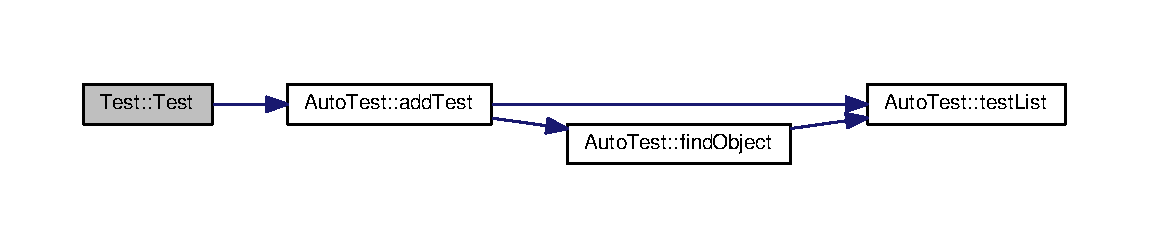
\includegraphics[width=350pt]{classTest_a744fa6648f5397560c203dc145146787_cgraph}
\end{center}
\end{figure}




\subsection{Member Data Documentation}
\hypertarget{classTest_acfb1db9d3c0e3f372aa716b6ead5a00c}{\index{Test@{Test}!child@{child}}
\index{child@{child}!Test@{Test}}
\subsubsection[{child}]{\setlength{\rightskip}{0pt plus 5cm}template$<$class T $>$ Q\-Shared\-Pointer$<$T$>$ {\bf Test}$<$ T $>$\-::child}}\label{classTest_acfb1db9d3c0e3f372aa716b6ead5a00c}


The documentation for this class was generated from the following file\-:\begin{DoxyCompactItemize}
\item 
\hyperlink{AutoTest_8h}{Auto\-Test.\-h}\end{DoxyCompactItemize}

\hypertarget{classTestCoord}{\section{Test\-Coord Class Reference}
\label{classTestCoord}\index{Test\-Coord@{Test\-Coord}}
}


{\ttfamily \#include $<$test\-\_\-coord.\-h$>$}



Inheritance diagram for Test\-Coord\-:
\nopagebreak
\begin{figure}[H]
\begin{center}
\leavevmode
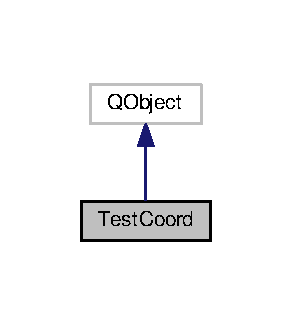
\includegraphics[width=140pt]{classTestCoord__inherit__graph}
\end{center}
\end{figure}


Collaboration diagram for Test\-Coord\-:
\nopagebreak
\begin{figure}[H]
\begin{center}
\leavevmode
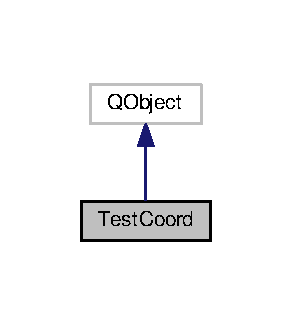
\includegraphics[width=140pt]{classTestCoord__coll__graph}
\end{center}
\end{figure}
\subsection*{Public Member Functions}
\begin{DoxyCompactItemize}
\item 
\hyperlink{classTestCoord_a59deda8ad0bc60d5a69fd16407b50583}{Test\-Coord} ()
\end{DoxyCompactItemize}


\subsection{Constructor \& Destructor Documentation}
\hypertarget{classTestCoord_a59deda8ad0bc60d5a69fd16407b50583}{\index{Test\-Coord@{Test\-Coord}!Test\-Coord@{Test\-Coord}}
\index{Test\-Coord@{Test\-Coord}!TestCoord@{Test\-Coord}}
\subsubsection[{Test\-Coord}]{\setlength{\rightskip}{0pt plus 5cm}Test\-Coord\-::\-Test\-Coord (
\begin{DoxyParamCaption}
{}
\end{DoxyParamCaption}
)}}\label{classTestCoord_a59deda8ad0bc60d5a69fd16407b50583}


The documentation for this class was generated from the following files\-:\begin{DoxyCompactItemize}
\item 
\hyperlink{test__coord_8h}{test\-\_\-coord.\-h}\item 
\hyperlink{test__coord_8cpp}{test\-\_\-coord.\-cpp}\end{DoxyCompactItemize}

\hypertarget{classTestRadar}{\section{Test\-Radar Class Reference}
\label{classTestRadar}\index{Test\-Radar@{Test\-Radar}}
}


{\ttfamily \#include $<$test\-\_\-radar.\-h$>$}



Inheritance diagram for Test\-Radar\-:
\nopagebreak
\begin{figure}[H]
\begin{center}
\leavevmode
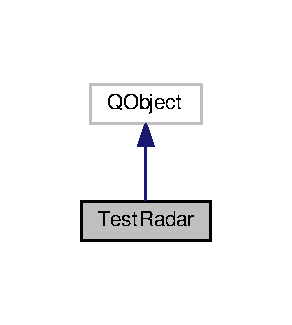
\includegraphics[width=140pt]{classTestRadar__inherit__graph}
\end{center}
\end{figure}


Collaboration diagram for Test\-Radar\-:
\nopagebreak
\begin{figure}[H]
\begin{center}
\leavevmode
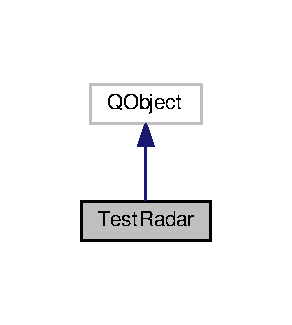
\includegraphics[width=140pt]{classTestRadar__coll__graph}
\end{center}
\end{figure}
\subsection*{Public Member Functions}
\begin{DoxyCompactItemize}
\item 
\hyperlink{classTestRadar_a447f28f55d7298648dfb7ab89b3f7466}{Test\-Radar} ()
\end{DoxyCompactItemize}


\subsection{Constructor \& Destructor Documentation}
\hypertarget{classTestRadar_a447f28f55d7298648dfb7ab89b3f7466}{\index{Test\-Radar@{Test\-Radar}!Test\-Radar@{Test\-Radar}}
\index{Test\-Radar@{Test\-Radar}!TestRadar@{Test\-Radar}}
\subsubsection[{Test\-Radar}]{\setlength{\rightskip}{0pt plus 5cm}Test\-Radar\-::\-Test\-Radar (
\begin{DoxyParamCaption}
{}
\end{DoxyParamCaption}
)}}\label{classTestRadar_a447f28f55d7298648dfb7ab89b3f7466}


The documentation for this class was generated from the following files\-:\begin{DoxyCompactItemize}
\item 
\hyperlink{test__radar_8h}{test\-\_\-radar.\-h}\item 
\hyperlink{test__radar_8cpp}{test\-\_\-radar.\-cpp}\end{DoxyCompactItemize}

\chapter{File Documentation}
\hypertarget{AutoTest_8h}{\section{Auto\-Test.\-h File Reference}
\label{AutoTest_8h}\index{Auto\-Test.\-h@{Auto\-Test.\-h}}
}
{\ttfamily \#include $<$Q\-Test$>$}\\*
{\ttfamily \#include $<$Q\-List$>$}\\*
{\ttfamily \#include $<$Q\-String$>$}\\*
{\ttfamily \#include $<$Q\-Shared\-Pointer$>$}\\*
Include dependency graph for Auto\-Test.\-h\-:
\nopagebreak
\begin{figure}[H]
\begin{center}
\leavevmode
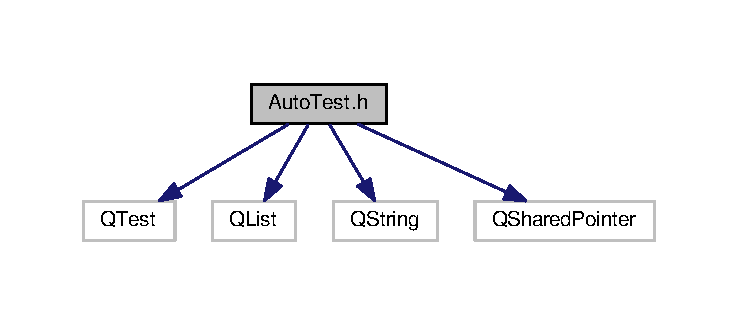
\includegraphics[width=350pt]{AutoTest_8h__incl}
\end{center}
\end{figure}
This graph shows which files directly or indirectly include this file\-:
\nopagebreak
\begin{figure}[H]
\begin{center}
\leavevmode
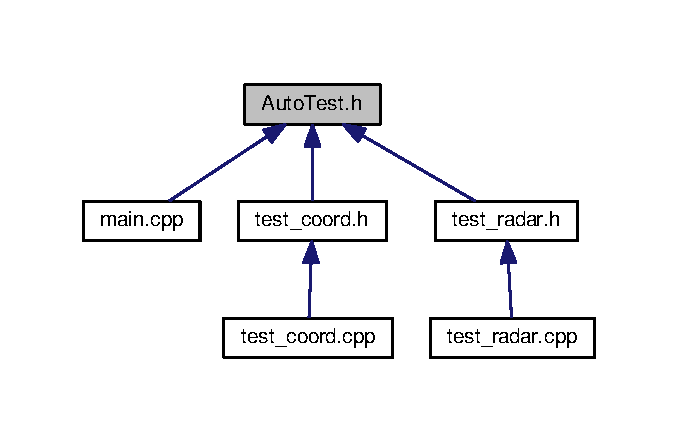
\includegraphics[width=325pt]{AutoTest_8h__dep__incl}
\end{center}
\end{figure}
\subsection*{Classes}
\begin{DoxyCompactItemize}
\item 
class \hyperlink{classTest}{Test$<$ T $>$}
\end{DoxyCompactItemize}
\subsection*{Namespaces}
\begin{DoxyCompactItemize}
\item 
\hyperlink{namespaceAutoTest}{Auto\-Test}
\end{DoxyCompactItemize}
\subsection*{Macros}
\begin{DoxyCompactItemize}
\item 
\#define \hyperlink{AutoTest_8h_a5247b55353f049080615de0a60b8133e}{D\-E\-C\-L\-A\-R\-E\-\_\-\-T\-E\-S\-T}(class\-Name)~static \hyperlink{classTest}{Test}$<$class\-Name$>$ t(\#class\-Name);
\item 
\#define \hyperlink{AutoTest_8h_a6ae82246e415b0258c23068cc7a4d5be}{T\-E\-S\-T\-\_\-\-M\-A\-I\-N}
\end{DoxyCompactItemize}
\subsection*{Typedefs}
\begin{DoxyCompactItemize}
\item 
typedef Q\-List$<$ Q\-Object $\ast$ $>$ \hyperlink{namespaceAutoTest_af30e241e62927ef8b429177cea542f2f}{Auto\-Test\-::\-Test\-List}
\end{DoxyCompactItemize}
\subsection*{Functions}
\begin{DoxyCompactItemize}
\item 
Test\-List \& \hyperlink{namespaceAutoTest_ad402cc96e71645ac9d583473f7ddbcd7}{Auto\-Test\-::test\-List} ()
\item 
bool \hyperlink{namespaceAutoTest_aebe87b1ec91a09f1b2739cbd4b301345}{Auto\-Test\-::find\-Object} (Q\-Object $\ast$object)
\item 
void \hyperlink{namespaceAutoTest_a3d2e7034d932dff0c2ba4170c442f594}{Auto\-Test\-::add\-Test} (Q\-Object $\ast$object)
\item 
int \hyperlink{namespaceAutoTest_a3261ec6bff9391a6f6779f63f6663b4b}{Auto\-Test\-::run} (int argc, char $\ast$argv\mbox{[}$\,$\mbox{]})
\end{DoxyCompactItemize}


\subsection{Macro Definition Documentation}
\hypertarget{AutoTest_8h_a5247b55353f049080615de0a60b8133e}{\index{Auto\-Test.\-h@{Auto\-Test.\-h}!D\-E\-C\-L\-A\-R\-E\-\_\-\-T\-E\-S\-T@{D\-E\-C\-L\-A\-R\-E\-\_\-\-T\-E\-S\-T}}
\index{D\-E\-C\-L\-A\-R\-E\-\_\-\-T\-E\-S\-T@{D\-E\-C\-L\-A\-R\-E\-\_\-\-T\-E\-S\-T}!AutoTest.h@{Auto\-Test.\-h}}
\subsubsection[{D\-E\-C\-L\-A\-R\-E\-\_\-\-T\-E\-S\-T}]{\setlength{\rightskip}{0pt plus 5cm}\#define D\-E\-C\-L\-A\-R\-E\-\_\-\-T\-E\-S\-T(
\begin{DoxyParamCaption}
\item[{}]{class\-Name}
\end{DoxyParamCaption}
)~static {\bf Test}$<$class\-Name$>$ t(\#class\-Name);}}\label{AutoTest_8h_a5247b55353f049080615de0a60b8133e}
\hypertarget{AutoTest_8h_a6ae82246e415b0258c23068cc7a4d5be}{\index{Auto\-Test.\-h@{Auto\-Test.\-h}!T\-E\-S\-T\-\_\-\-M\-A\-I\-N@{T\-E\-S\-T\-\_\-\-M\-A\-I\-N}}
\index{T\-E\-S\-T\-\_\-\-M\-A\-I\-N@{T\-E\-S\-T\-\_\-\-M\-A\-I\-N}!AutoTest.h@{Auto\-Test.\-h}}
\subsubsection[{T\-E\-S\-T\-\_\-\-M\-A\-I\-N}]{\setlength{\rightskip}{0pt plus 5cm}\#define T\-E\-S\-T\-\_\-\-M\-A\-I\-N}}\label{AutoTest_8h_a6ae82246e415b0258c23068cc7a4d5be}
{\bfseries Value\-:}
\begin{DoxyCode}
\textcolor{keywordtype}{int} \hyperlink{main_8cpp_a0ddf1224851353fc92bfbff6f499fa97}{main}(\textcolor{keywordtype}{int} argc, \textcolor{keywordtype}{char} *argv[]) \(\backslash\)
    \{ \(\backslash\)
      return \hyperlink{namespaceAutoTest_a3261ec6bff9391a6f6779f63f6663b4b}{AutoTest::run}(argc, argv); \(\backslash\)
  \}
\end{DoxyCode}

\hypertarget{coords_8cpp}{\section{coords.\-cpp File Reference}
\label{coords_8cpp}\index{coords.\-cpp@{coords.\-cpp}}
}


Tento subor obsahuje konstruktor a metody triedy \hyperlink{classCoords}{Coords} predstavujuce suradnice radaroveho systemu.  


{\ttfamily \#include \char`\"{}coords.\-h\char`\"{}}\\*
Include dependency graph for coords.\-cpp\-:
\nopagebreak
\begin{figure}[H]
\begin{center}
\leavevmode
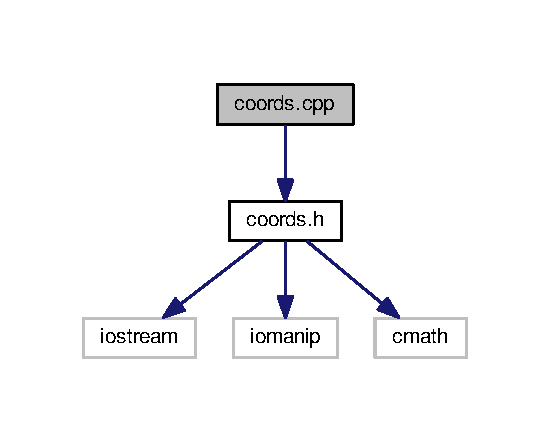
\includegraphics[width=264pt]{coords_8cpp__incl}
\end{center}
\end{figure}
\subsection*{Functions}
\begin{DoxyCompactItemize}
\item 
{\footnotesize template$<$typename T $>$ }\\T \hyperlink{coords_8cpp_a53e268e712f4977619c54a41fd762536}{sgn} (T n)
\end{DoxyCompactItemize}


\subsection{Detailed Description}
Tento subor obsahuje konstruktor a metody triedy \hyperlink{classCoords}{Coords} predstavujuce suradnice radaroveho systemu. Mozny obsahlejsi popis na vice radek. 

\subsection{Function Documentation}
\hypertarget{coords_8cpp_a53e268e712f4977619c54a41fd762536}{\index{coords.\-cpp@{coords.\-cpp}!sgn@{sgn}}
\index{sgn@{sgn}!coords.cpp@{coords.\-cpp}}
\subsubsection[{sgn}]{\setlength{\rightskip}{0pt plus 5cm}template$<$typename T $>$ T sgn (
\begin{DoxyParamCaption}
\item[{T}]{n}
\end{DoxyParamCaption}
)}}\label{coords_8cpp_a53e268e712f4977619c54a41fd762536}

\hypertarget{coords_8h}{\section{coords.\-h File Reference}
\label{coords_8h}\index{coords.\-h@{coords.\-h}}
}
{\ttfamily \#include $<$iostream$>$}\\*
{\ttfamily \#include $<$iomanip$>$}\\*
{\ttfamily \#include $<$cmath$>$}\\*
Include dependency graph for coords.\-h\-:
\nopagebreak
\begin{figure}[H]
\begin{center}
\leavevmode
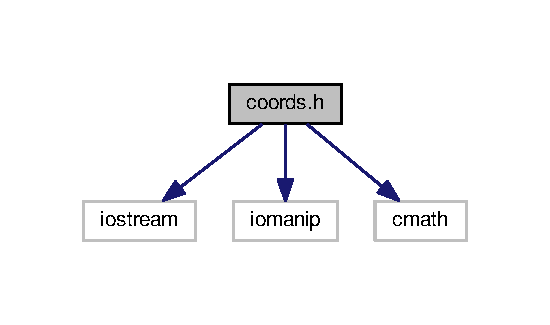
\includegraphics[width=264pt]{coords_8h__incl}
\end{center}
\end{figure}
This graph shows which files directly or indirectly include this file\-:
\nopagebreak
\begin{figure}[H]
\begin{center}
\leavevmode
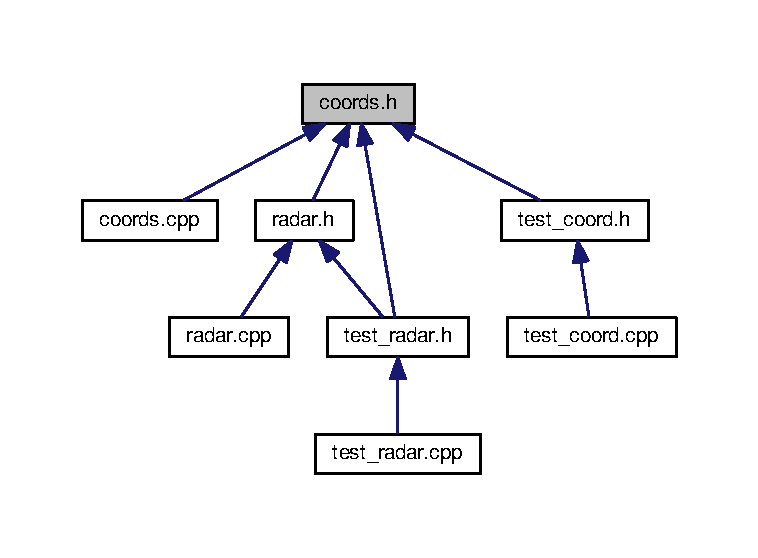
\includegraphics[width=350pt]{coords_8h__dep__incl}
\end{center}
\end{figure}
\subsection*{Classes}
\begin{DoxyCompactItemize}
\item 
class \hyperlink{classCoords}{Coords}
\begin{DoxyCompactList}\small\item\em Trieda \hyperlink{classCoords}{Coords}. \end{DoxyCompactList}\end{DoxyCompactItemize}

\hypertarget{main_8cpp}{\section{main.\-cpp File Reference}
\label{main_8cpp}\index{main.\-cpp@{main.\-cpp}}
}
{\ttfamily \#include $<$Q\-Core\-Application$>$}\\*
{\ttfamily \#include \char`\"{}Auto\-Test.\-h\char`\"{}}\\*
{\ttfamily \#include $<$Q\-Debug$>$}\\*
Include dependency graph for main.\-cpp\-:
\nopagebreak
\begin{figure}[H]
\begin{center}
\leavevmode
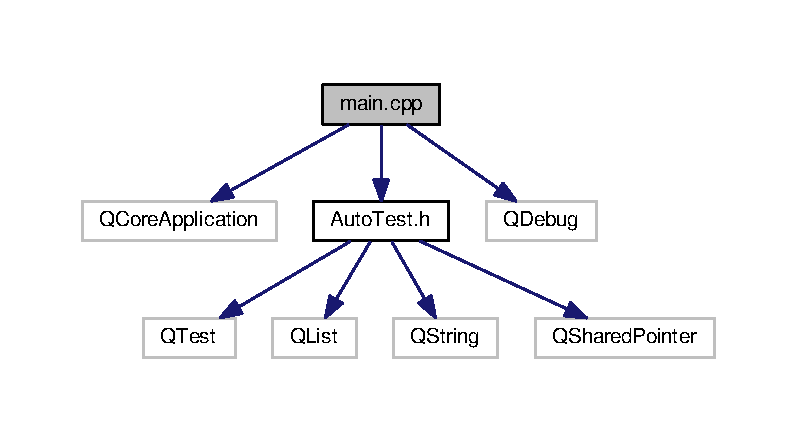
\includegraphics[width=350pt]{main_8cpp__incl}
\end{center}
\end{figure}
\subsection*{Functions}
\begin{DoxyCompactItemize}
\item 
int \hyperlink{main_8cpp_a0ddf1224851353fc92bfbff6f499fa97}{main} (int argc, char $\ast$argv\mbox{[}$\,$\mbox{]})
\end{DoxyCompactItemize}


\subsection{Function Documentation}
\hypertarget{main_8cpp_a0ddf1224851353fc92bfbff6f499fa97}{\index{main.\-cpp@{main.\-cpp}!main@{main}}
\index{main@{main}!main.cpp@{main.\-cpp}}
\subsubsection[{main}]{\setlength{\rightskip}{0pt plus 5cm}int main (
\begin{DoxyParamCaption}
\item[{int}]{argc, }
\item[{char $\ast$}]{argv\mbox{[}$\,$\mbox{]}}
\end{DoxyParamCaption}
)}}\label{main_8cpp_a0ddf1224851353fc92bfbff6f499fa97}


Here is the call graph for this function\-:
\nopagebreak
\begin{figure}[H]
\begin{center}
\leavevmode
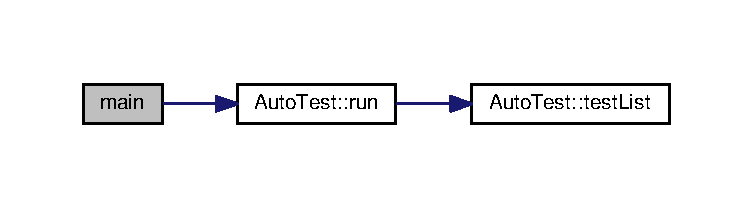
\includegraphics[width=350pt]{main_8cpp_a0ddf1224851353fc92bfbff6f499fa97_cgraph}
\end{center}
\end{figure}



\hypertarget{radar_8cpp}{\section{radar.\-cpp File Reference}
\label{radar_8cpp}\index{radar.\-cpp@{radar.\-cpp}}
}
{\ttfamily \#include \char`\"{}radar.\-h\char`\"{}}\\*
Include dependency graph for radar.\-cpp\-:
\nopagebreak
\begin{figure}[H]
\begin{center}
\leavevmode
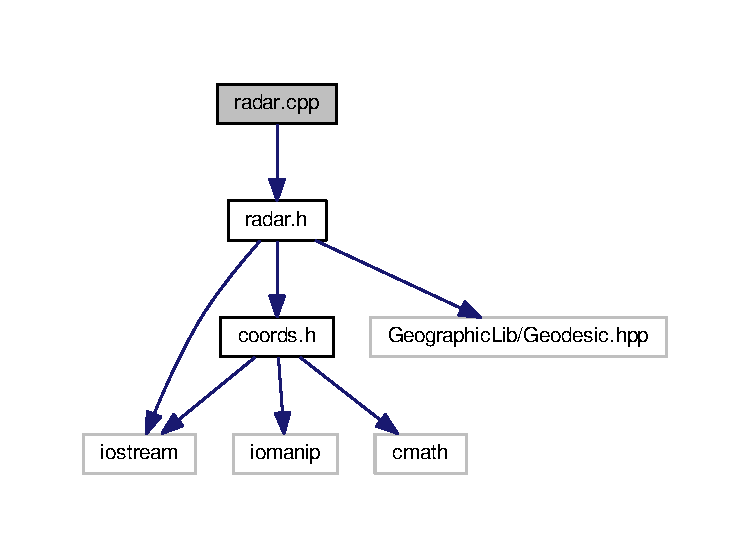
\includegraphics[width=350pt]{radar_8cpp__incl}
\end{center}
\end{figure}

\hypertarget{radar_8h}{\section{radar.\-h File Reference}
\label{radar_8h}\index{radar.\-h@{radar.\-h}}
}
{\ttfamily \#include \char`\"{}coords.\-h\char`\"{}}\\*
{\ttfamily \#include $<$iostream$>$}\\*
{\ttfamily \#include $<$Geographic\-Lib/\-Geodesic.\-hpp$>$}\\*
Include dependency graph for radar.\-h\-:
\nopagebreak
\begin{figure}[H]
\begin{center}
\leavevmode
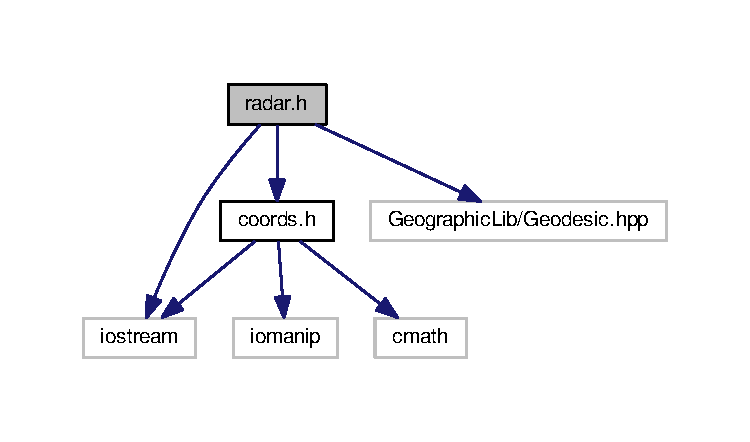
\includegraphics[width=350pt]{radar_8h__incl}
\end{center}
\end{figure}
This graph shows which files directly or indirectly include this file\-:
\nopagebreak
\begin{figure}[H]
\begin{center}
\leavevmode
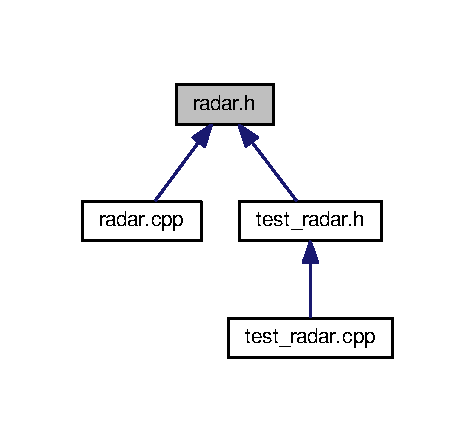
\includegraphics[width=228pt]{radar_8h__dep__incl}
\end{center}
\end{figure}
\subsection*{Classes}
\begin{DoxyCompactItemize}
\item 
class \hyperlink{classRadar}{Radar}
\begin{DoxyCompactList}\small\item\em Trieda \hyperlink{classRadar}{Radar}. \end{DoxyCompactList}\end{DoxyCompactItemize}

\hypertarget{test__coord_8cpp}{\section{test\-\_\-coord.\-cpp File Reference}
\label{test__coord_8cpp}\index{test\-\_\-coord.\-cpp@{test\-\_\-coord.\-cpp}}
}
{\ttfamily \#include \char`\"{}test\-\_\-coord.\-h\char`\"{}}\\*
Include dependency graph for test\-\_\-coord.\-cpp\-:
\nopagebreak
\begin{figure}[H]
\begin{center}
\leavevmode
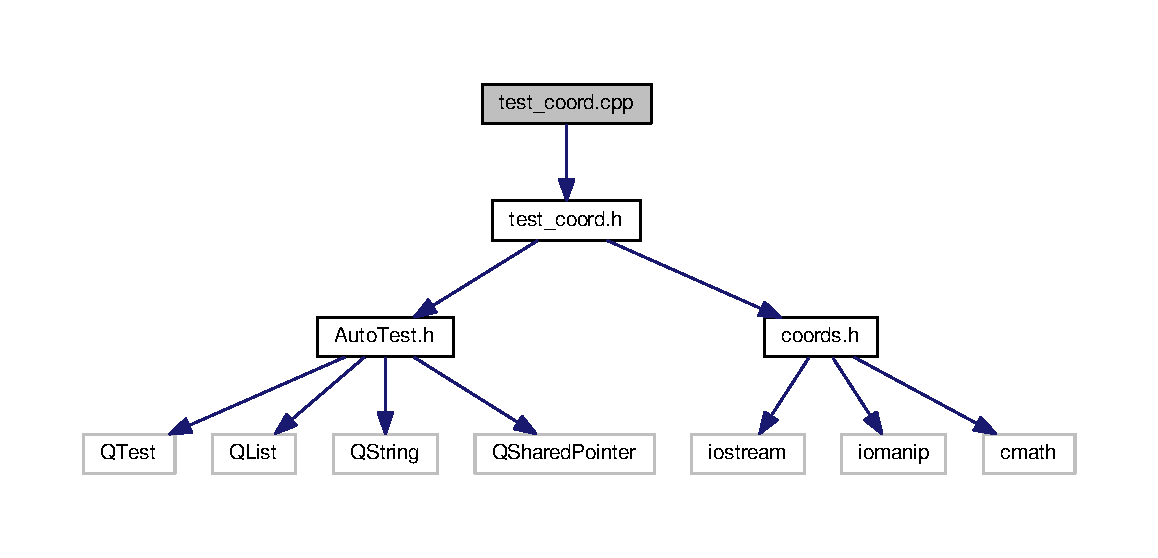
\includegraphics[width=350pt]{test__coord_8cpp__incl}
\end{center}
\end{figure}
\subsection*{Functions}
\begin{DoxyCompactItemize}
\item 
double \hyperlink{test__coord_8cpp_a744b6f7c221775ca99c9757c1e905a34}{cut\-Number} (double number)
\end{DoxyCompactItemize}
\subsection*{Variables}
\begin{DoxyCompactItemize}
\item 
double \hyperlink{test__coord_8cpp_aac22643c72d9b0007638f778e7f9cf4c}{cut\-Dec\-Lat}
\item 
double \hyperlink{test__coord_8cpp_abf2325470a525cf070f8ac0870125e2d}{cut\-Dec\-Long}
\item 
\hyperlink{classCoords}{Coords} \hyperlink{test__coord_8cpp_a535c564fe3bb5e813482c3898dd8ac5e}{mssr\-\_\-veljav} (48, 15, 38.\-56, 17, 9, 47.\-83)
\item 
\hyperlink{classCoords}{Coords} \hyperlink{test__coord_8cpp_a403bc11659ca226668b9b96f1dd46c7d}{mssr\-\_\-bucen} (48, 18, 19.\-95, 19, 52, 14.\-61)
\item 
\hyperlink{classCoords}{Coords} \hyperlink{test__coord_8cpp_abc5852178071a9910854009e2517b716}{mie\-\_\-mor} (48, 3, 42.\-00, 17, 22, 35.\-00)
\item 
\hyperlink{classCoords}{Coords} \hyperlink{test__coord_8cpp_a8138a535d73212a15f0db5337fb1e6e1}{mich\-\_\-p37} (48, 43, 24.\-98, 21, 57, 4.\-39)
\item 
\hyperlink{classCoords}{Coords} \hyperlink{test__coord_8cpp_a10271582d1f211287476add5f0628353}{po\-\_\-mor5} (49, 1, 55.\-2701, 21, 18, 51.\-607)
\end{DoxyCompactItemize}


\subsection{Function Documentation}
\hypertarget{test__coord_8cpp_a744b6f7c221775ca99c9757c1e905a34}{\index{test\-\_\-coord.\-cpp@{test\-\_\-coord.\-cpp}!cut\-Number@{cut\-Number}}
\index{cut\-Number@{cut\-Number}!test_coord.cpp@{test\-\_\-coord.\-cpp}}
\subsubsection[{cut\-Number}]{\setlength{\rightskip}{0pt plus 5cm}double cut\-Number (
\begin{DoxyParamCaption}
\item[{double}]{number}
\end{DoxyParamCaption}
)}}\label{test__coord_8cpp_a744b6f7c221775ca99c9757c1e905a34}


\subsection{Variable Documentation}
\hypertarget{test__coord_8cpp_aac22643c72d9b0007638f778e7f9cf4c}{\index{test\-\_\-coord.\-cpp@{test\-\_\-coord.\-cpp}!cut\-Dec\-Lat@{cut\-Dec\-Lat}}
\index{cut\-Dec\-Lat@{cut\-Dec\-Lat}!test_coord.cpp@{test\-\_\-coord.\-cpp}}
\subsubsection[{cut\-Dec\-Lat}]{\setlength{\rightskip}{0pt plus 5cm}double cut\-Dec\-Lat}}\label{test__coord_8cpp_aac22643c72d9b0007638f778e7f9cf4c}
\hypertarget{test__coord_8cpp_abf2325470a525cf070f8ac0870125e2d}{\index{test\-\_\-coord.\-cpp@{test\-\_\-coord.\-cpp}!cut\-Dec\-Long@{cut\-Dec\-Long}}
\index{cut\-Dec\-Long@{cut\-Dec\-Long}!test_coord.cpp@{test\-\_\-coord.\-cpp}}
\subsubsection[{cut\-Dec\-Long}]{\setlength{\rightskip}{0pt plus 5cm}double cut\-Dec\-Long}}\label{test__coord_8cpp_abf2325470a525cf070f8ac0870125e2d}
\hypertarget{test__coord_8cpp_a8138a535d73212a15f0db5337fb1e6e1}{\index{test\-\_\-coord.\-cpp@{test\-\_\-coord.\-cpp}!mich\-\_\-p37@{mich\-\_\-p37}}
\index{mich\-\_\-p37@{mich\-\_\-p37}!test_coord.cpp@{test\-\_\-coord.\-cpp}}
\subsubsection[{mich\-\_\-p37}]{\setlength{\rightskip}{0pt plus 5cm}{\bf Coords} mich\-\_\-p37(48, 43, 24.\-98, 21, 57, 4.\-39)}}\label{test__coord_8cpp_a8138a535d73212a15f0db5337fb1e6e1}
\hypertarget{test__coord_8cpp_abc5852178071a9910854009e2517b716}{\index{test\-\_\-coord.\-cpp@{test\-\_\-coord.\-cpp}!mie\-\_\-mor@{mie\-\_\-mor}}
\index{mie\-\_\-mor@{mie\-\_\-mor}!test_coord.cpp@{test\-\_\-coord.\-cpp}}
\subsubsection[{mie\-\_\-mor}]{\setlength{\rightskip}{0pt plus 5cm}{\bf Coords} mie\-\_\-mor(48, 3, 42.\-00, 17, 22, 35.\-00)}}\label{test__coord_8cpp_abc5852178071a9910854009e2517b716}
\hypertarget{test__coord_8cpp_a403bc11659ca226668b9b96f1dd46c7d}{\index{test\-\_\-coord.\-cpp@{test\-\_\-coord.\-cpp}!mssr\-\_\-bucen@{mssr\-\_\-bucen}}
\index{mssr\-\_\-bucen@{mssr\-\_\-bucen}!test_coord.cpp@{test\-\_\-coord.\-cpp}}
\subsubsection[{mssr\-\_\-bucen}]{\setlength{\rightskip}{0pt plus 5cm}{\bf Coords} mssr\-\_\-bucen(48, 18, 19.\-95, 19, 52, 14.\-61)}}\label{test__coord_8cpp_a403bc11659ca226668b9b96f1dd46c7d}
\hypertarget{test__coord_8cpp_a535c564fe3bb5e813482c3898dd8ac5e}{\index{test\-\_\-coord.\-cpp@{test\-\_\-coord.\-cpp}!mssr\-\_\-veljav@{mssr\-\_\-veljav}}
\index{mssr\-\_\-veljav@{mssr\-\_\-veljav}!test_coord.cpp@{test\-\_\-coord.\-cpp}}
\subsubsection[{mssr\-\_\-veljav}]{\setlength{\rightskip}{0pt plus 5cm}{\bf Coords} mssr\-\_\-veljav(48, 15, 38.\-56, 17, 9, 47.\-83)}}\label{test__coord_8cpp_a535c564fe3bb5e813482c3898dd8ac5e}
\hypertarget{test__coord_8cpp_a10271582d1f211287476add5f0628353}{\index{test\-\_\-coord.\-cpp@{test\-\_\-coord.\-cpp}!po\-\_\-mor5@{po\-\_\-mor5}}
\index{po\-\_\-mor5@{po\-\_\-mor5}!test_coord.cpp@{test\-\_\-coord.\-cpp}}
\subsubsection[{po\-\_\-mor5}]{\setlength{\rightskip}{0pt plus 5cm}{\bf Coords} po\-\_\-mor5(49, 1, 55.\-2701, 21, 18, 51.\-607)}}\label{test__coord_8cpp_a10271582d1f211287476add5f0628353}

\hypertarget{test__coord_8h}{\section{test\-\_\-coord.\-h File Reference}
\label{test__coord_8h}\index{test\-\_\-coord.\-h@{test\-\_\-coord.\-h}}
}
{\ttfamily \#include \char`\"{}Auto\-Test.\-h\char`\"{}}\\*
{\ttfamily \#include \char`\"{}coords.\-h\char`\"{}}\\*
Include dependency graph for test\-\_\-coord.\-h\-:
\nopagebreak
\begin{figure}[H]
\begin{center}
\leavevmode
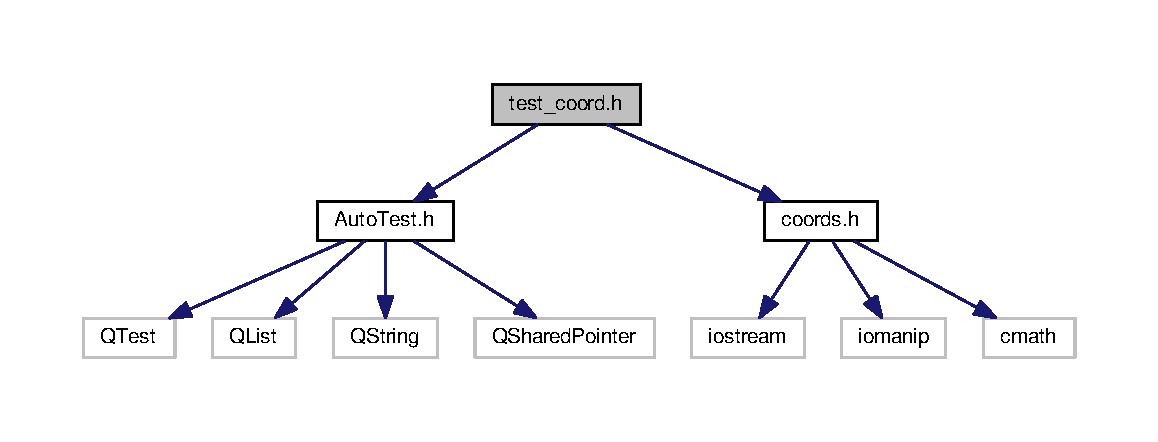
\includegraphics[width=350pt]{test__coord_8h__incl}
\end{center}
\end{figure}
This graph shows which files directly or indirectly include this file\-:
\nopagebreak
\begin{figure}[H]
\begin{center}
\leavevmode
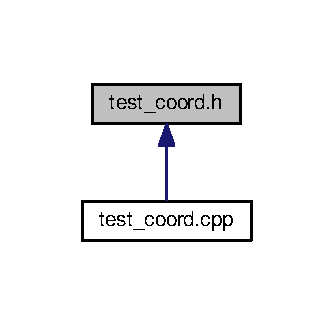
\includegraphics[width=160pt]{test__coord_8h__dep__incl}
\end{center}
\end{figure}
\subsection*{Classes}
\begin{DoxyCompactItemize}
\item 
class \hyperlink{classTestCoord}{Test\-Coord}
\end{DoxyCompactItemize}

\hypertarget{test__radar_8cpp}{\section{test\-\_\-radar.\-cpp File Reference}
\label{test__radar_8cpp}\index{test\-\_\-radar.\-cpp@{test\-\_\-radar.\-cpp}}
}
{\ttfamily \#include \char`\"{}test\-\_\-radar.\-h\char`\"{}}\\*
Include dependency graph for test\-\_\-radar.\-cpp\-:
\nopagebreak
\begin{figure}[H]
\begin{center}
\leavevmode
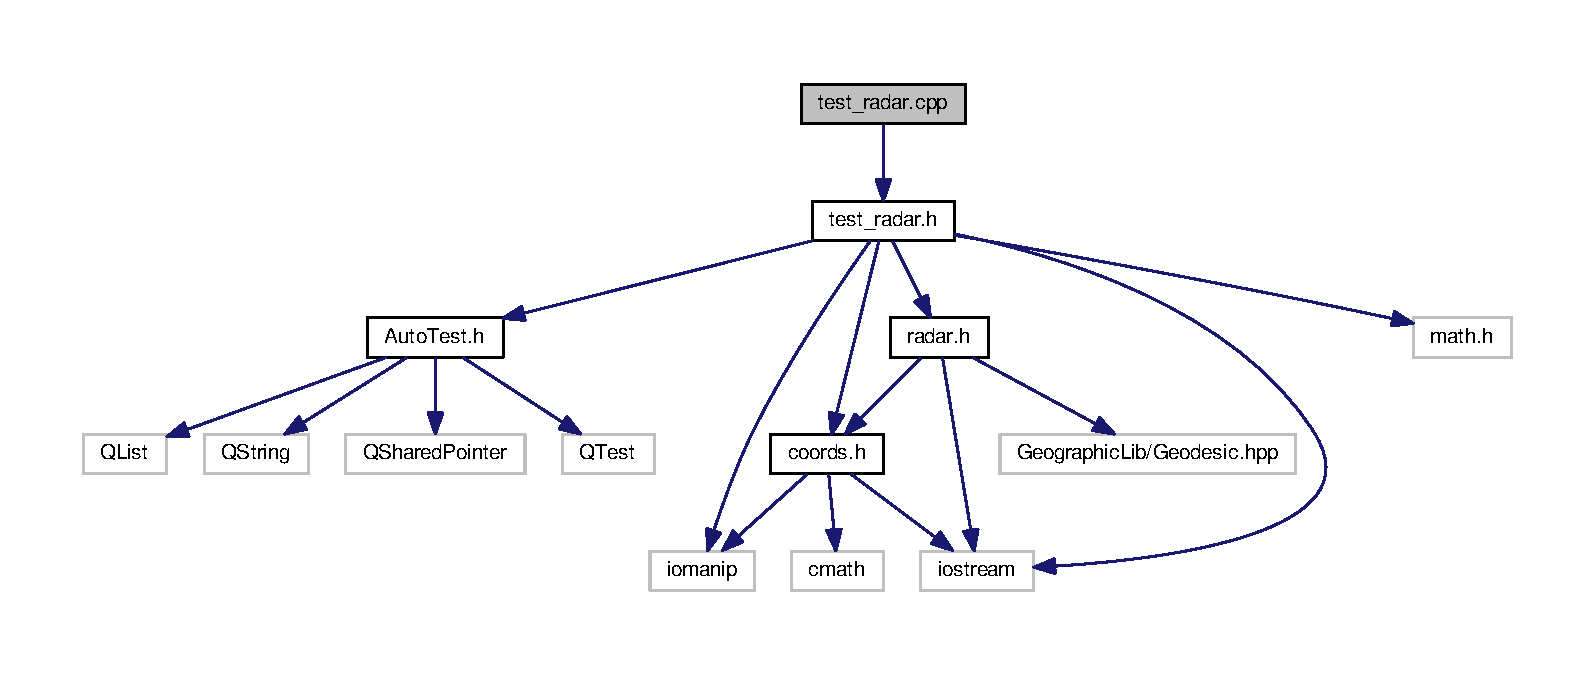
\includegraphics[width=350pt]{test__radar_8cpp__incl}
\end{center}
\end{figure}
\subsection*{Variables}
\begin{DoxyCompactItemize}
\item 
\hyperlink{classCoords}{Coords} \hyperlink{test__radar_8cpp_af1771fb2ed9f14625a2d887457ac34dd}{mssr\-\_\-\-\_\-veljav} (48, 15, 38.\-56, 17, 9, 47.\-83)
\item 
\hyperlink{classCoords}{Coords} \hyperlink{test__radar_8cpp_a9b2ad95951b755e225be5d5576ef73b3}{mssr\-\_\-\-\_\-bucen} (48, 18, 19.\-95, 19, 52, 14.\-61)
\item 
\hyperlink{classCoords}{Coords} \hyperlink{test__radar_8cpp_aa27430fff1af4c588b55983d640c5ded}{mie\-\_\-\-\_\-mor} (48, 3, 42.\-00, 17, 22, 35.\-00)
\item 
\hyperlink{classCoords}{Coords} \hyperlink{test__radar_8cpp_a2101a262e1771c5171ad21f6524be191}{mich\-\_\-\-\_\-p37} (48, 43, 24.\-98, 21, 57, 4.\-39)
\item 
\hyperlink{classCoords}{Coords} \hyperlink{test__radar_8cpp_a32d3fdddfb6e17e997215d37f7cc8473}{po\-\_\-\-\_\-mor5} (49, 1, 55.\-2701, 21, 18, 51.\-607)
\item 
\hyperlink{classRadar}{Radar} \hyperlink{test__radar_8cpp_a32c8e4a85355b96214a05fccf6ab6eed}{r1} (\hyperlink{test__radar_8cpp_af1771fb2ed9f14625a2d887457ac34dd}{mssr\-\_\-\-\_\-veljav}, \hyperlink{test__radar_8cpp_a9b2ad95951b755e225be5d5576ef73b3}{mssr\-\_\-\-\_\-bucen})
\end{DoxyCompactItemize}


\subsection{Variable Documentation}
\hypertarget{test__radar_8cpp_a2101a262e1771c5171ad21f6524be191}{\index{test\-\_\-radar.\-cpp@{test\-\_\-radar.\-cpp}!mich\-\_\-\-\_\-p37@{mich\-\_\-\-\_\-p37}}
\index{mich\-\_\-\-\_\-p37@{mich\-\_\-\-\_\-p37}!test_radar.cpp@{test\-\_\-radar.\-cpp}}
\subsubsection[{mich\-\_\-\-\_\-p37}]{\setlength{\rightskip}{0pt plus 5cm}{\bf Coords} mich\-\_\-\-\_\-p37(48, 43, 24.\-98, 21, 57, 4.\-39)}}\label{test__radar_8cpp_a2101a262e1771c5171ad21f6524be191}
\hypertarget{test__radar_8cpp_aa27430fff1af4c588b55983d640c5ded}{\index{test\-\_\-radar.\-cpp@{test\-\_\-radar.\-cpp}!mie\-\_\-\-\_\-mor@{mie\-\_\-\-\_\-mor}}
\index{mie\-\_\-\-\_\-mor@{mie\-\_\-\-\_\-mor}!test_radar.cpp@{test\-\_\-radar.\-cpp}}
\subsubsection[{mie\-\_\-\-\_\-mor}]{\setlength{\rightskip}{0pt plus 5cm}{\bf Coords} mie\-\_\-\-\_\-mor(48, 3, 42.\-00, 17, 22, 35.\-00)}}\label{test__radar_8cpp_aa27430fff1af4c588b55983d640c5ded}
\hypertarget{test__radar_8cpp_a9b2ad95951b755e225be5d5576ef73b3}{\index{test\-\_\-radar.\-cpp@{test\-\_\-radar.\-cpp}!mssr\-\_\-\-\_\-bucen@{mssr\-\_\-\-\_\-bucen}}
\index{mssr\-\_\-\-\_\-bucen@{mssr\-\_\-\-\_\-bucen}!test_radar.cpp@{test\-\_\-radar.\-cpp}}
\subsubsection[{mssr\-\_\-\-\_\-bucen}]{\setlength{\rightskip}{0pt plus 5cm}{\bf Coords} mssr\-\_\-\-\_\-bucen(48, 18, 19.\-95, 19, 52, 14.\-61)}}\label{test__radar_8cpp_a9b2ad95951b755e225be5d5576ef73b3}
\hypertarget{test__radar_8cpp_af1771fb2ed9f14625a2d887457ac34dd}{\index{test\-\_\-radar.\-cpp@{test\-\_\-radar.\-cpp}!mssr\-\_\-\-\_\-veljav@{mssr\-\_\-\-\_\-veljav}}
\index{mssr\-\_\-\-\_\-veljav@{mssr\-\_\-\-\_\-veljav}!test_radar.cpp@{test\-\_\-radar.\-cpp}}
\subsubsection[{mssr\-\_\-\-\_\-veljav}]{\setlength{\rightskip}{0pt plus 5cm}{\bf Coords} mssr\-\_\-\-\_\-veljav(48, 15, 38.\-56, 17, 9, 47.\-83)}}\label{test__radar_8cpp_af1771fb2ed9f14625a2d887457ac34dd}
\hypertarget{test__radar_8cpp_a32d3fdddfb6e17e997215d37f7cc8473}{\index{test\-\_\-radar.\-cpp@{test\-\_\-radar.\-cpp}!po\-\_\-\-\_\-mor5@{po\-\_\-\-\_\-mor5}}
\index{po\-\_\-\-\_\-mor5@{po\-\_\-\-\_\-mor5}!test_radar.cpp@{test\-\_\-radar.\-cpp}}
\subsubsection[{po\-\_\-\-\_\-mor5}]{\setlength{\rightskip}{0pt plus 5cm}{\bf Coords} po\-\_\-\-\_\-mor5(49, 1, 55.\-2701, 21, 18, 51.\-607)}}\label{test__radar_8cpp_a32d3fdddfb6e17e997215d37f7cc8473}
\hypertarget{test__radar_8cpp_a32c8e4a85355b96214a05fccf6ab6eed}{\index{test\-\_\-radar.\-cpp@{test\-\_\-radar.\-cpp}!r1@{r1}}
\index{r1@{r1}!test_radar.cpp@{test\-\_\-radar.\-cpp}}
\subsubsection[{r1}]{\setlength{\rightskip}{0pt plus 5cm}{\bf Radar} r1({\bf mssr\-\_\-\-\_\-veljav}, {\bf mssr\-\_\-\-\_\-bucen})}}\label{test__radar_8cpp_a32c8e4a85355b96214a05fccf6ab6eed}

\hypertarget{test__radar_8h}{\section{test\-\_\-radar.\-h File Reference}
\label{test__radar_8h}\index{test\-\_\-radar.\-h@{test\-\_\-radar.\-h}}
}
{\ttfamily \#include \char`\"{}Auto\-Test.\-h\char`\"{}}\\*
{\ttfamily \#include \char`\"{}coords.\-h\char`\"{}}\\*
{\ttfamily \#include \char`\"{}radar.\-h\char`\"{}}\\*
{\ttfamily \#include $<$math.\-h$>$}\\*
{\ttfamily \#include $<$iomanip$>$}\\*
{\ttfamily \#include $<$iostream$>$}\\*
Include dependency graph for test\-\_\-radar.\-h\-:
\nopagebreak
\begin{figure}[H]
\begin{center}
\leavevmode
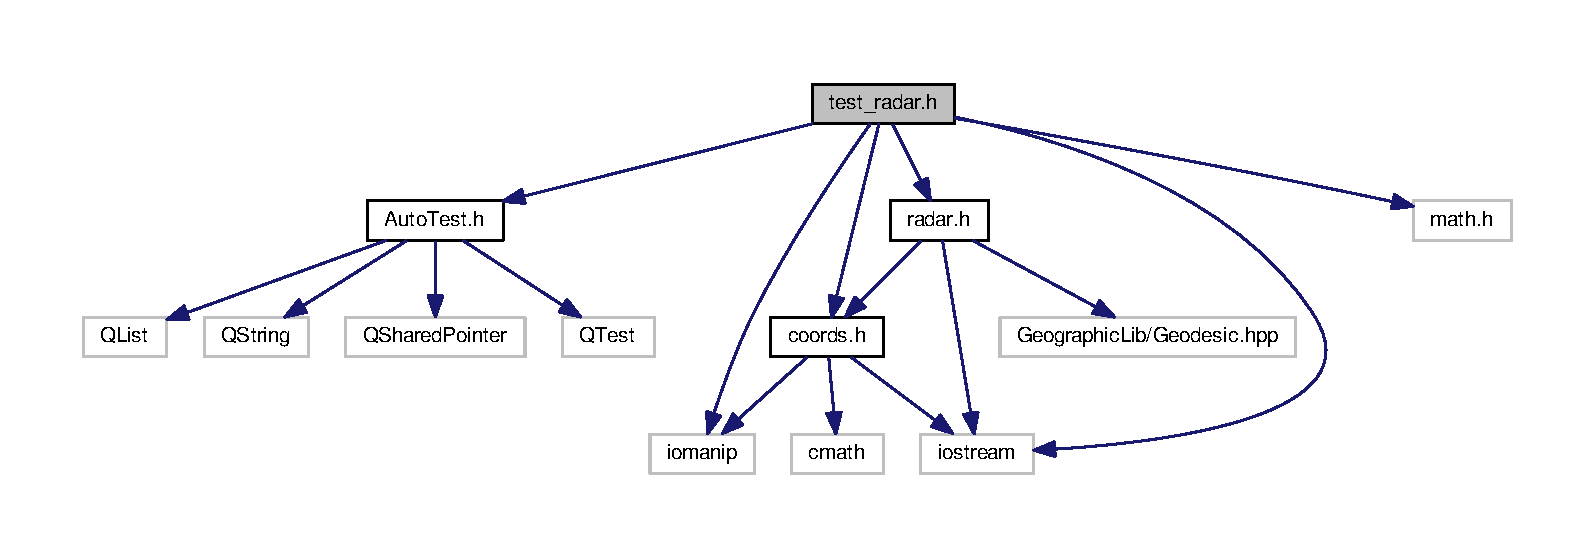
\includegraphics[width=350pt]{test__radar_8h__incl}
\end{center}
\end{figure}
This graph shows which files directly or indirectly include this file\-:
\nopagebreak
\begin{figure}[H]
\begin{center}
\leavevmode
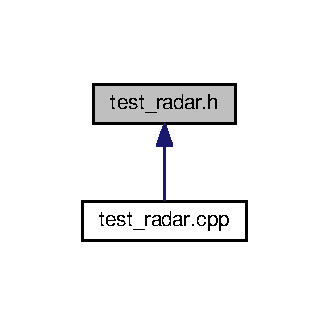
\includegraphics[width=158pt]{test__radar_8h__dep__incl}
\end{center}
\end{figure}
\subsection*{Classes}
\begin{DoxyCompactItemize}
\item 
class \hyperlink{classTestRadar}{Test\-Radar}
\end{DoxyCompactItemize}

%--- End generated contents ---

% Index
\newpage
\phantomsection
\addcontentsline{toc}{chapter}{Index}
\printindex

\end{document}
